%% Background Theory
%%=========================================

\chapter{Background Theory}
\label{ch:background}
\red{TODO}

%%=========================================

\section{General Neural Network}
\red{Must be rewritten slighylt}. At the base of the neural machine translation systems are neural networks. The idea of models using artificial neurons, can be traced back to the 1940s. Since then, more sophisticated proposals and variants have been made from decade to decade. Artificial neural networks are an attempt at modeling the information process capabilities of nervous systems, found in the brain. This is done by implementing mathematical models of neurons \citep{russell2010aimodernapproach}.

\begin{figure}[ht]
    \centering
    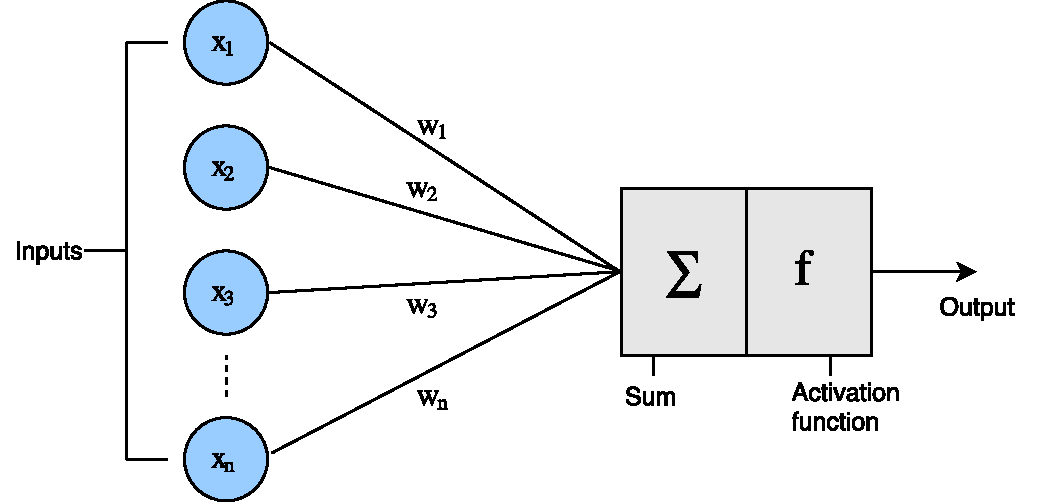
\includegraphics[width=0.8\textwidth]{fig/related_work/nn_perceptron.pdf}
    \caption{Illustration of a mathematical model of a neuron}
    \label{fig:nn-perceptron}
\end{figure}

Figure \ref{fig:nn-rnn} illustrates a simple mathematical model for a neuron, often called a unit or a node. This unit ``fires" when a linear combination of its inputs exceeds some threshold. A neural network is a collection of many such units. The properties of a network is determined by its topology, as well as the properties of the units. Networks are constructed by directly linking nodes with each other. A link from unit \(i\) to unit \(j\) serves to propagate the activation \(a_{i}\) from \(i\) to \(j\). The strength and sign of the signal is determined by the numeric weight that is associated with the unit. A feed-forward network consists of units which has connections that only goes in one direction. These node receives input from the ``upstream" nodes, and delivers output to the ``downstream" nodes, forming a directed acyclic graph \citep{russell2010aimodernapproach}.

%%=========================================

\section{Recurrent Neural Network}
Another way to construct a neural network is by using loops. A recurrent neural network \citep{rumelhart1988learning} is a network much like a feed-forward network, but in addition to feeding ``downstream" nodes, nodes also feeds its output back into its own inputs. This type of architecture can support a short-term memory, a feature that is necessary in problems where input also depends on previous input \citep{russell2010aimodernapproach}. For example would such characteristics be necessary if we fed the network words in a sentence, and we asked the network to predict the next word it had not yet seen. 

\begin{figure}[ht]
    \centering
    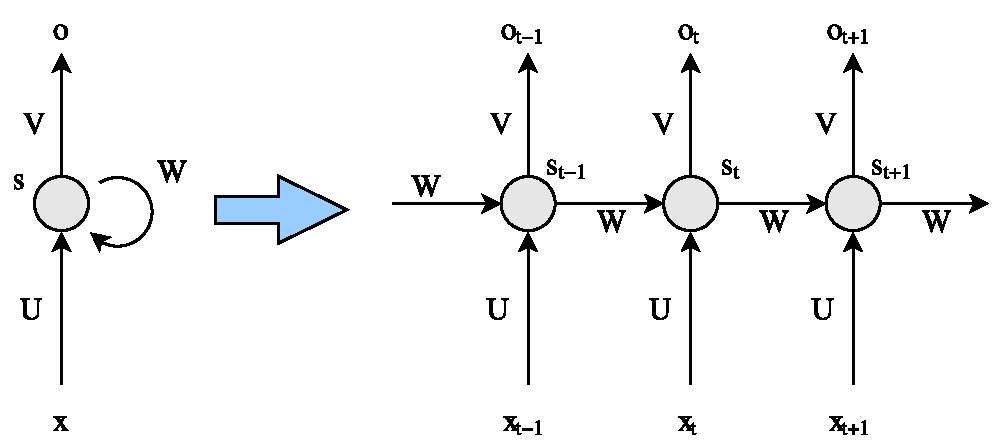
\includegraphics[width=0.7\textwidth]{fig/related_work/nn_recurrent.pdf}
    \caption{A compact and an unfolded recurrent neural network}
    \label{fig:nn-rnn}
\end{figure}

We can consider RNNs as a type of loop, and we can also unfold it into a complete sequence, as illustrated in Figure \ref{fig:nn-rnn}. In the figure, \(x_{t}\) is the input, and \(s_{t}\) is the hidden state of the recurrent network at time step \(t\). The hidden state functions as its memory as it is reused in the next time step, along with the input of the current time step. It is also important to note that the network shares the same weights \(W\) across several time steps.The recurrent neural network has input to hidden connections parametrized by a weight matrix \(U\), as well as hidden-to-hidden recurrent connections parametrized by a weight matrix \(W\). In addition, the network has hidden-to-output connection parametrized by a weight matrix \(V\) \citep{goodfellow2016deeplearning}.

\begin{align}
    \begin{split}\label{eq:rnn-eq-1}
        h_{t}&=\sigma(b+Ws_{t-1}+Ux_{t})
    \end{split}\\
    \begin{split}\label{eq:rnn-eq-2}
        \hat{y_{t}}&=\sigma(c+Vh_{t})
    \end{split}
\end{align}

Equations \ref{eq:rnn-eq-1} and \ref{eq:rnn-eq-2} are slightly modified from \citep{goodfellow2016deeplearning}, and defines the forward propagation of the model illustrated in Figure \ref{fig:nn-rnn}. The parameters \(b\) and \(c\) are the bias vectors. Computing the gradient in a recurrent neural network is done with a back-propagation algorithm called back-propagation through time \citep{werbos1990backpropagation}. 

%%=========================================

\section{Long-Short Term Memory}
The Long-Short Term Memory (LSTM) is a recurrent neural network architecture. It was first purposed by \citep{hochreiter1997long}, and was meant to address some of the shortcomings of more basic recurrent neural network architectures. \citep{bengio1994learning} showed that recurrent neural network faced an increasingly difficult problem as the duration of the dependencies to be captures increases. While the architecture could take into account short-term dependencies rather well, long-term dependencies were increasingly difficult to learn. The LSTMs were explicitly designed to avoid the long-term dependency problem. 

\begin{figure}[ht]
    \centering
    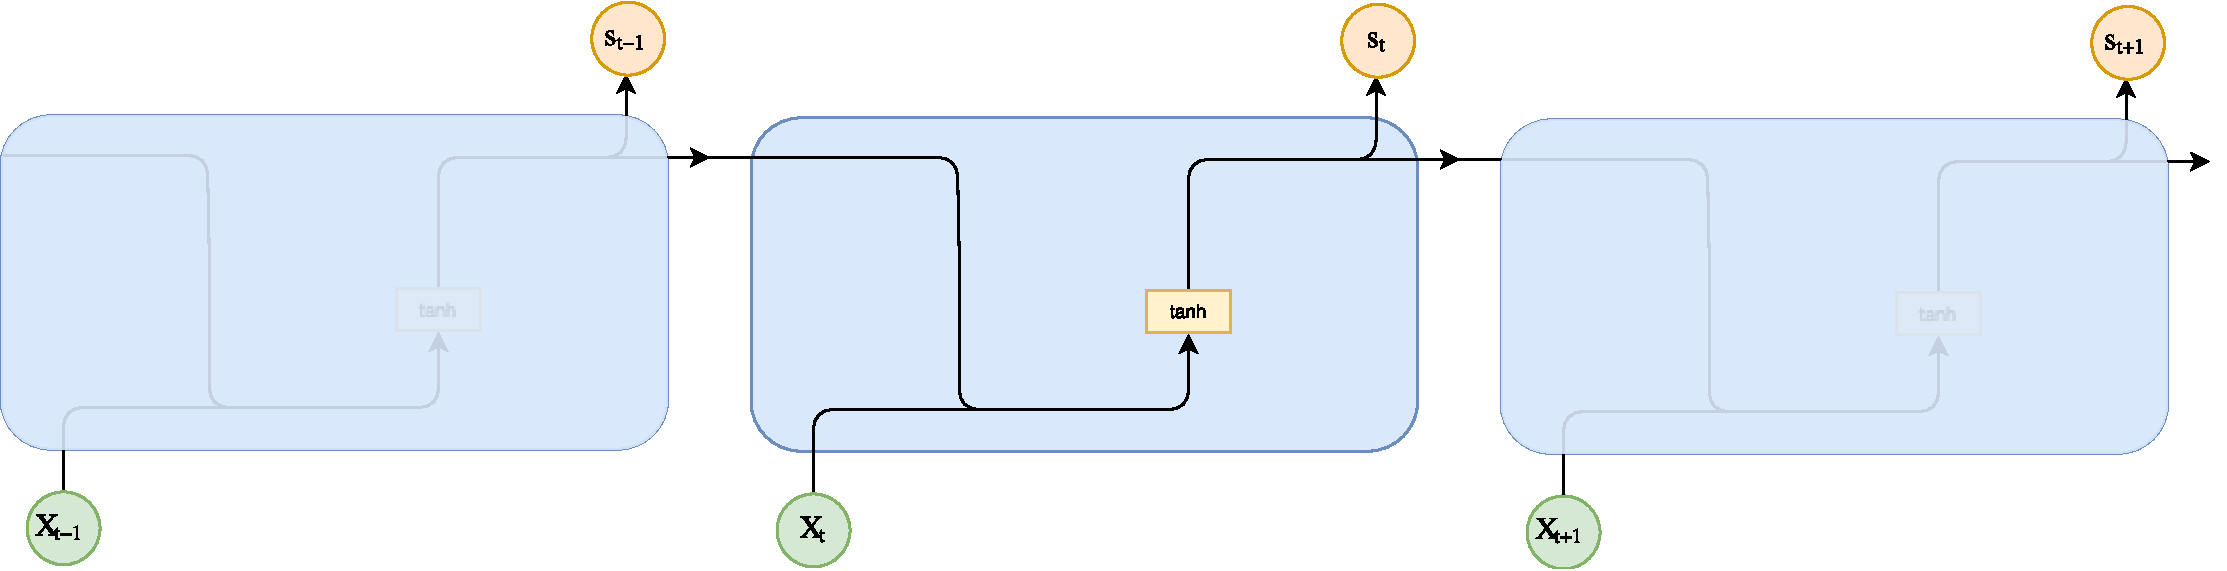
\includegraphics[width=1\textwidth]{fig/related_work/rnn_flow.pdf}
    \caption{Flow of a standard RNN}
    \label{fig:nn-rnn-flow}
\end{figure}

Figure \ref{fig:nn-rnn-flow} illustrates the chain like structure of standard recurrent neural network. Its architecture is relatively simple, containing only one layer. In this illustration our layer uses the hyperbolic tangent function (tanh).

\begin{figure}[ht]
    \centering
    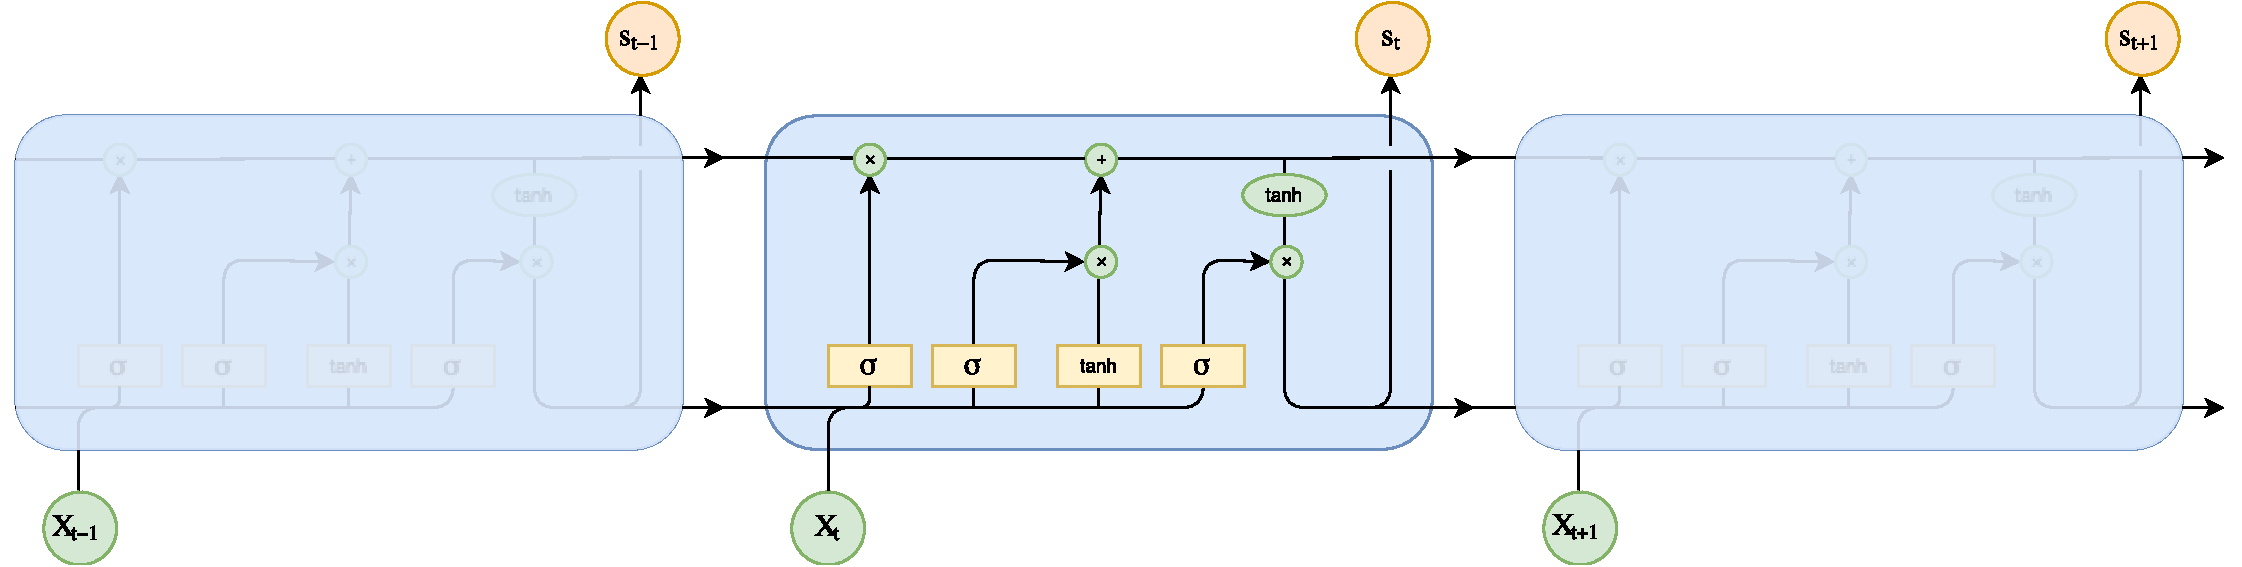
\includegraphics[width=1\textwidth]{fig/related_work/lstm_flow.pdf}
    \caption{Flow of a LSTM cell}
    \label{fig:nn-lstm-flow}
\end{figure}

Figure \ref{fig:nn-lstm-flow} illustrates a similar chain structure, but that of a LSTM cell. The LSTM module has a different structure, and instead of having a single neural network layer, like the simpler RNN, it has four layers. The topmost horizontal line carries the cell state of the unit. The LSTM unit is enriched by several co-called gating units. These gates regulate what information is remembered by the cell state, and what is forgotten. The leftmost sigmoid layer is called the ``forget gate layer". This gate decides what the state should forgotten from the existing information. The next sigmoid gate is called the ``input gate layer" and determines which values should be updated. The hyperbolic tangent gate layer creates a vector of candidate values, which could be added to the cell state. After the state is updated, or the candidate is thrown away, the final sigmoid gate, the ``output gate layer" decides what the parts of the cell state should be outputted \citep{hochreiter1997long, goodfellow2016deeplearning, olah2015lstm, gers2002learning}.